% Options for packages loaded elsewhere
\PassOptionsToPackage{unicode}{hyperref}
\PassOptionsToPackage{hyphens}{url}
\PassOptionsToPackage{dvipsnames,svgnames,x11names}{xcolor}
%
\documentclass[
  letterpaper,
  DIV=11,
  numbers=noendperiod]{scrartcl}

\usepackage{amsmath,amssymb}
\usepackage{iftex}
\ifPDFTeX
  \usepackage[T1]{fontenc}
  \usepackage[utf8]{inputenc}
  \usepackage{textcomp} % provide euro and other symbols
\else % if luatex or xetex
  \usepackage{unicode-math}
  \defaultfontfeatures{Scale=MatchLowercase}
  \defaultfontfeatures[\rmfamily]{Ligatures=TeX,Scale=1}
\fi
\usepackage{lmodern}
\ifPDFTeX\else  
    % xetex/luatex font selection
\fi
% Use upquote if available, for straight quotes in verbatim environments
\IfFileExists{upquote.sty}{\usepackage{upquote}}{}
\IfFileExists{microtype.sty}{% use microtype if available
  \usepackage[]{microtype}
  \UseMicrotypeSet[protrusion]{basicmath} % disable protrusion for tt fonts
}{}
\makeatletter
\@ifundefined{KOMAClassName}{% if non-KOMA class
  \IfFileExists{parskip.sty}{%
    \usepackage{parskip}
  }{% else
    \setlength{\parindent}{0pt}
    \setlength{\parskip}{6pt plus 2pt minus 1pt}}
}{% if KOMA class
  \KOMAoptions{parskip=half}}
\makeatother
\usepackage{xcolor}
\setlength{\emergencystretch}{3em} % prevent overfull lines
\setcounter{secnumdepth}{5}
% Make \paragraph and \subparagraph free-standing
\ifx\paragraph\undefined\else
  \let\oldparagraph\paragraph
  \renewcommand{\paragraph}[1]{\oldparagraph{#1}\mbox{}}
\fi
\ifx\subparagraph\undefined\else
  \let\oldsubparagraph\subparagraph
  \renewcommand{\subparagraph}[1]{\oldsubparagraph{#1}\mbox{}}
\fi


\providecommand{\tightlist}{%
  \setlength{\itemsep}{0pt}\setlength{\parskip}{0pt}}\usepackage{longtable,booktabs,array}
\usepackage{calc} % for calculating minipage widths
% Correct order of tables after \paragraph or \subparagraph
\usepackage{etoolbox}
\makeatletter
\patchcmd\longtable{\par}{\if@noskipsec\mbox{}\fi\par}{}{}
\makeatother
% Allow footnotes in longtable head/foot
\IfFileExists{footnotehyper.sty}{\usepackage{footnotehyper}}{\usepackage{footnote}}
\makesavenoteenv{longtable}
\usepackage{graphicx}
\makeatletter
\def\maxwidth{\ifdim\Gin@nat@width>\linewidth\linewidth\else\Gin@nat@width\fi}
\def\maxheight{\ifdim\Gin@nat@height>\textheight\textheight\else\Gin@nat@height\fi}
\makeatother
% Scale images if necessary, so that they will not overflow the page
% margins by default, and it is still possible to overwrite the defaults
% using explicit options in \includegraphics[width, height, ...]{}
\setkeys{Gin}{width=\maxwidth,height=\maxheight,keepaspectratio}
% Set default figure placement to htbp
\makeatletter
\def\fps@figure{htbp}
\makeatother
\newlength{\cslhangindent}
\setlength{\cslhangindent}{1.5em}
\newlength{\csllabelwidth}
\setlength{\csllabelwidth}{3em}
\newlength{\cslentryspacingunit} % times entry-spacing
\setlength{\cslentryspacingunit}{\parskip}
\newenvironment{CSLReferences}[2] % #1 hanging-ident, #2 entry spacing
 {% don't indent paragraphs
  \setlength{\parindent}{0pt}
  % turn on hanging indent if param 1 is 1
  \ifodd #1
  \let\oldpar\par
  \def\par{\hangindent=\cslhangindent\oldpar}
  \fi
  % set entry spacing
  \setlength{\parskip}{#2\cslentryspacingunit}
 }%
 {}
\usepackage{calc}
\newcommand{\CSLBlock}[1]{#1\hfill\break}
\newcommand{\CSLLeftMargin}[1]{\parbox[t]{\csllabelwidth}{#1}}
\newcommand{\CSLRightInline}[1]{\parbox[t]{\linewidth - \csllabelwidth}{#1}\break}
\newcommand{\CSLIndent}[1]{\hspace{\cslhangindent}#1}

\usepackage{booktabs}
\usepackage{longtable}
\usepackage{array}
\usepackage{multirow}
\usepackage{wrapfig}
\usepackage{float}
\usepackage{colortbl}
\usepackage{pdflscape}
\usepackage{tabu}
\usepackage{threeparttable}
\usepackage{threeparttablex}
\usepackage[normalem]{ulem}
\usepackage{makecell}
\usepackage{xcolor}
\KOMAoption{captions}{tableheading}
\makeatletter
\makeatother
\makeatletter
\makeatother
\makeatletter
\@ifpackageloaded{caption}{}{\usepackage{caption}}
\AtBeginDocument{%
\ifdefined\contentsname
  \renewcommand*\contentsname{Table of contents}
\else
  \newcommand\contentsname{Table of contents}
\fi
\ifdefined\listfigurename
  \renewcommand*\listfigurename{List of Figures}
\else
  \newcommand\listfigurename{List of Figures}
\fi
\ifdefined\listtablename
  \renewcommand*\listtablename{List of Tables}
\else
  \newcommand\listtablename{List of Tables}
\fi
\ifdefined\figurename
  \renewcommand*\figurename{Figure}
\else
  \newcommand\figurename{Figure}
\fi
\ifdefined\tablename
  \renewcommand*\tablename{Table}
\else
  \newcommand\tablename{Table}
\fi
}
\@ifpackageloaded{float}{}{\usepackage{float}}
\floatstyle{ruled}
\@ifundefined{c@chapter}{\newfloat{codelisting}{h}{lop}}{\newfloat{codelisting}{h}{lop}[chapter]}
\floatname{codelisting}{Listing}
\newcommand*\listoflistings{\listof{codelisting}{List of Listings}}
\makeatother
\makeatletter
\@ifpackageloaded{caption}{}{\usepackage{caption}}
\@ifpackageloaded{subcaption}{}{\usepackage{subcaption}}
\makeatother
\makeatletter
\@ifpackageloaded{tcolorbox}{}{\usepackage[skins,breakable]{tcolorbox}}
\makeatother
\makeatletter
\@ifundefined{shadecolor}{\definecolor{shadecolor}{rgb}{.97, .97, .97}}
\makeatother
\makeatletter
\makeatother
\makeatletter
\makeatother
\ifLuaTeX
  \usepackage{selnolig}  % disable illegal ligatures
\fi
\IfFileExists{bookmark.sty}{\usepackage{bookmark}}{\usepackage{hyperref}}
\IfFileExists{xurl.sty}{\usepackage{xurl}}{} % add URL line breaks if available
\urlstyle{same} % disable monospaced font for URLs
\hypersetup{
  pdftitle={My title},
  pdfauthor={Jeongwoo Kim; Jiwon Choi},
  colorlinks=true,
  linkcolor={blue},
  filecolor={Maroon},
  citecolor={Blue},
  urlcolor={Blue},
  pdfcreator={LaTeX via pandoc}}

\title{My title\thanks{Code and data are available at:
https://github.com/Kjeongwoo99/STA302H\_Paper3}}
\usepackage{etoolbox}
\makeatletter
\providecommand{\subtitle}[1]{% add subtitle to \maketitle
  \apptocmd{\@title}{\par {\large #1 \par}}{}{}
}
\makeatother
\subtitle{My subtitle if needed}
\author{Jeongwoo Kim \and Jiwon Choi}
\date{March 13, 2024}

\begin{document}
\maketitle
\begin{abstract}
First sentence. Second sentence. Third sentence. Fourth sentence.
\end{abstract}
\ifdefined\Shaded\renewenvironment{Shaded}{\begin{tcolorbox}[breakable, interior hidden, frame hidden, enhanced, sharp corners, boxrule=0pt, borderline west={3pt}{0pt}{shadecolor}]}{\end{tcolorbox}}\fi

\hypertarget{introduction}{%
\section{Introduction}\label{introduction}}

You can and should cross-reference sections and sub-sections. We use R
Core Team (2023) and Wickham et al. (2019).

The remainder of this paper is structured as follows.
Section~\ref{sec-data}\ldots.

\hypertarget{sec-data}{%
\section{Data}\label{sec-data}}

We have used two datasets for this study. One is the U.S election survey
data of Democracy Fund + UCLA Nationscape dataset from the Voter Study
Group, conducted on October 3, 2019. Second is the census data from
IPUMS America Census Service, which is used as the post-stratification
data for the survey data to adjust the weight.

\hypertarget{survey-data}{%
\subsection{Survey Data}\label{survey-data}}

This survey data is an 18-month election study conducted by UCLA
researchers with roughly 6250 online interviews each from from July 2019
to February 2021 (Tausanovitch and Vavreck (2020)). The sample is
weighted to represent the U.S. adult population (Tausanovitch and
Vavreck (2020)). Nationscape groups weight on the following important
factors: gender, the four major census regions, race, Hispanic
ethnicity, household income, education, age, language spoken at home,
nativity, 2016 presidential vote, and the urban-rural mix of the
respondent's ZIP code (Tausanovitch and Vavreck (2020)). According to
the data, Male make up 48.3\% while female make up 51.3\% (Tausanovitch
and Vavreck (2020)). 74.2\% of the respondents are White, 6.8\% are
Asian/Pacific, 12\% are Black (Tausanovitch and Vavreck (2020)). 20.4\%
are those between 18-29, 33.4\% are 30-49, 32.4\% are 50-69, 3.3\% are
70+ (Tausanovitch and Vavreck (2020)). On average, 5.1 percent declined
immediately among those who are selected for the survey. 16.7 percent of
the respondents did not complete the survey. Another 5.9 percent were
categorized as speeding or straight-line which means they completed the
survey in less than 6 minutes or selected the same response for every
question in the three policy question batteries. Leaving these out leave
72.4 percent of the original sample for the analysis.

The Nationscape survey's strength lies in its methodological rigor - the
effectiveness in collecting large samples from the U.S. citizen and its
weighting strategy desinged to mirror the U.S. adult population by
including weight factors such as age, gender, race and income and more.
As they filter out inaccurate or missing data, it makes sure that the
data collected are accurate and ensures data integrity. While other
datasets such as the General Social Survey (GSS) and the American
National Election Studies (ANES) are available, the Nationscape
dataset's frequency (surveys collected every week) give it an advantage
in analyzing electoral trends and shifts in real-time. Its' extensive
sample size also justifies the choice of this dataset.

For our analysis, we decided to focus on five demographics: age, gender,
education, race and state. Age is important because in general, voters
tend to become more conservative as they get older. To account for the
age difference, we divided the age group into four categories: 18-29,
30-49, 50-69 and 70+.

Gender is also an important category because in general, men tend be
more conservative and women tend to be more liberal. Recently, gender
issues are growing social issues and this may affect the election, hence
we wanted to explore how this affects our model.

Education is also an interesting factor. In the past, non-college white
voters used to support Democrats while college-educated white voters
supported Republicans (Harris (2018)). However, there has been a switch
in this trend as 61 percent of non-college white voters showed their
support wheres just 45 percent of college-educated white voters did in
the exit polls (Harris (2018)). Only 37 percent of those without a
degree cast their votes for Democrats while 53 percent with a degree did
so (Harris (2018)). We categorized education into four categories: `High
school or less', `Some college', `College degree', `Postgrad'.

Race also needs some attention because normally non-white groups are
highly in favour of Democrats regardless of candidates and white swing
by depending on candidates. According to the statistics collected in
2016, 93\% of black, 71\% of Latino, 68\% of Asian support democrats
while only 41\% of white support democrats (Prokop (2021)). As white
voters make up 74\% of the voting population, it is really important for
both parties to attain this demographic group.

Lastly, states are very important as some states historically favor
conservatives while some states vote for democrats. In general, the west
and the east coasts are democrat supporters whereas south are
conservative supporters.

\hypertarget{post-stratification-data}{%
\subsection{Post-stratification Data}\label{post-stratification-data}}

IPUMS (``Integrated Public Use Microdata Series'') is a website that
offers database of samples of the American population from the American
Community Surveys of 2000-present. These samples provide rich
qualitative information on the long-term changes in the population. We
selected the '\,' data as the post-stratification dataset for our
research. The ACS is an ongoing survey that collects data monthly, which
is then combined into 1-year, 3-year, and 5-year aggregates. It then
uses stratified sampling where the U.S population is broken down into
sub-groups and initial weights are assigned to each respondent.

One strength of the IPUMS survey is the fact that it provides a
comprehensive and extensive data with detailed demographic of the U.S.
population with social, economic and housing characteristics, which is
very useful in our analysis of the 2020 U.S presidential election
forecast. The longitudinal data of this survey also allows researchers
to analyze trends over time. The U.S. Census Bureau offers credibility
of the data with high quality checks. The post-stratification process
ensures correcting for sampling biases and non-response. On the other
hand, since the survey relies on self-report, there lies a risk of
response bias inherently. While it is an ongoing survey, there is still
a time lag between the data collection and data availability. However,
the large sample size, consistency and reliability of the data
collection, the integrated data over time with post-stratification can
justify the decision to utilize IPUMS data over other sources.

The variables we have decided to use in this analysis from the dataset
are `sex', `race', `stateicp', `age\_group', and `educd'. We have
filtered out the respondents who have answered `other' or no available
sex data from the raw dataset for simplicity of the analysis. Therefore,
`Sex' is categorized into `Male' and `Female'. `Race' is divided into
`White', `Black', `Asian', `American Indian' and `Other'. As mentioned
earlier, the fact that white, black and Asian together make up around 93
percent of the U.S population, this categorization is justified.
`stateicp' is a record of all the states in the U.S. We have used the
abbreviations for each state, for example, `CT' for Connecticut, `ME'
for Maine, `MA' for Massachusetts. We have the data of 55 states in
total. `age\_group' categorized the respondents' age into four groups:
`18-29', `30-49', `50-64' and `65+'. `education' is divided into four
categories: `High school or less', `Some college', `College degree',
`Postgrad'. We filtered out those unknowns, and cleaned the dataset by
assigning each respondent to the right category accordingly.

\begin{figure}

{\centering 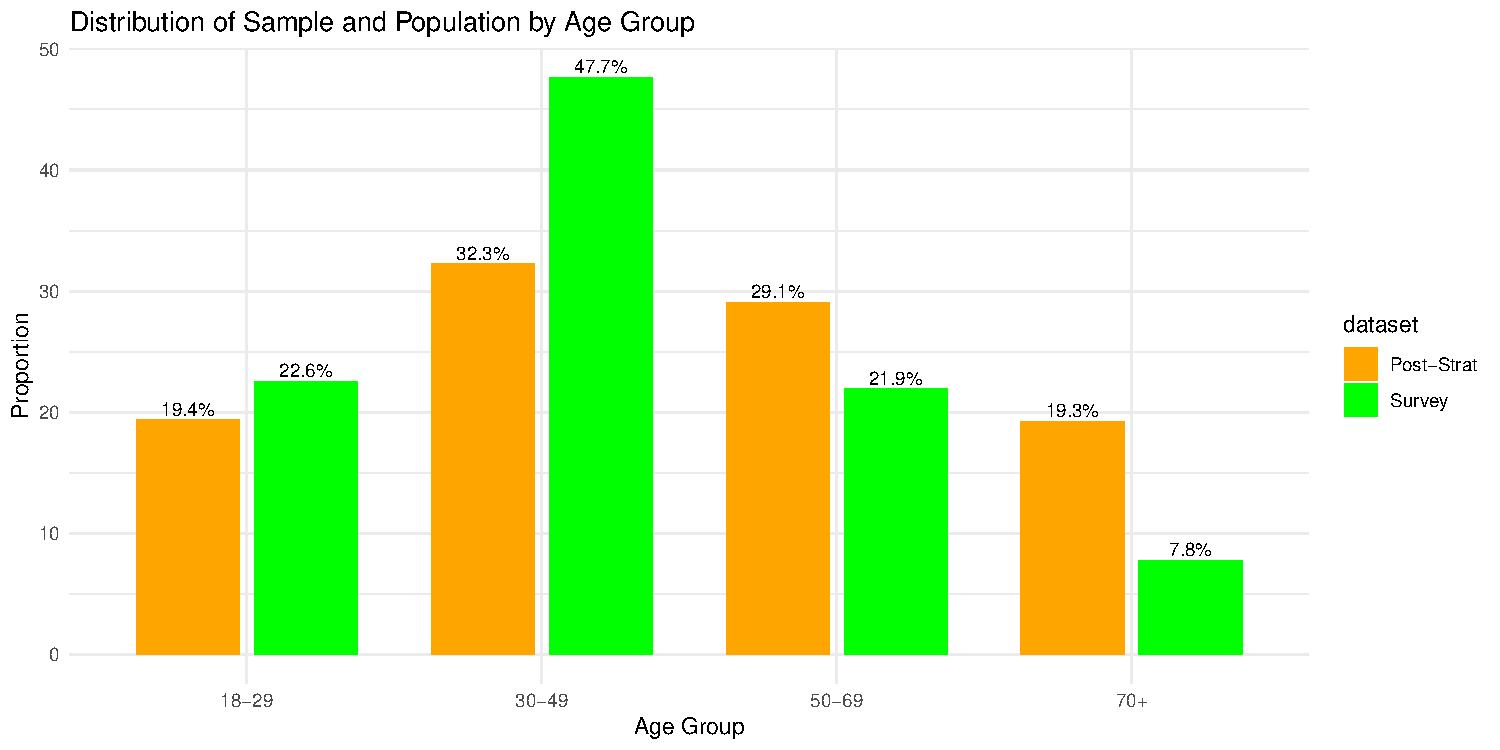
\includegraphics{paper_files/figure-pdf/fig-distribution-by-age-group-1.pdf}

}

\caption{\label{fig-distribution-by-age-group}Distribution of Sample and
Population by Age Group}

\end{figure}

\begin{figure}

{\centering 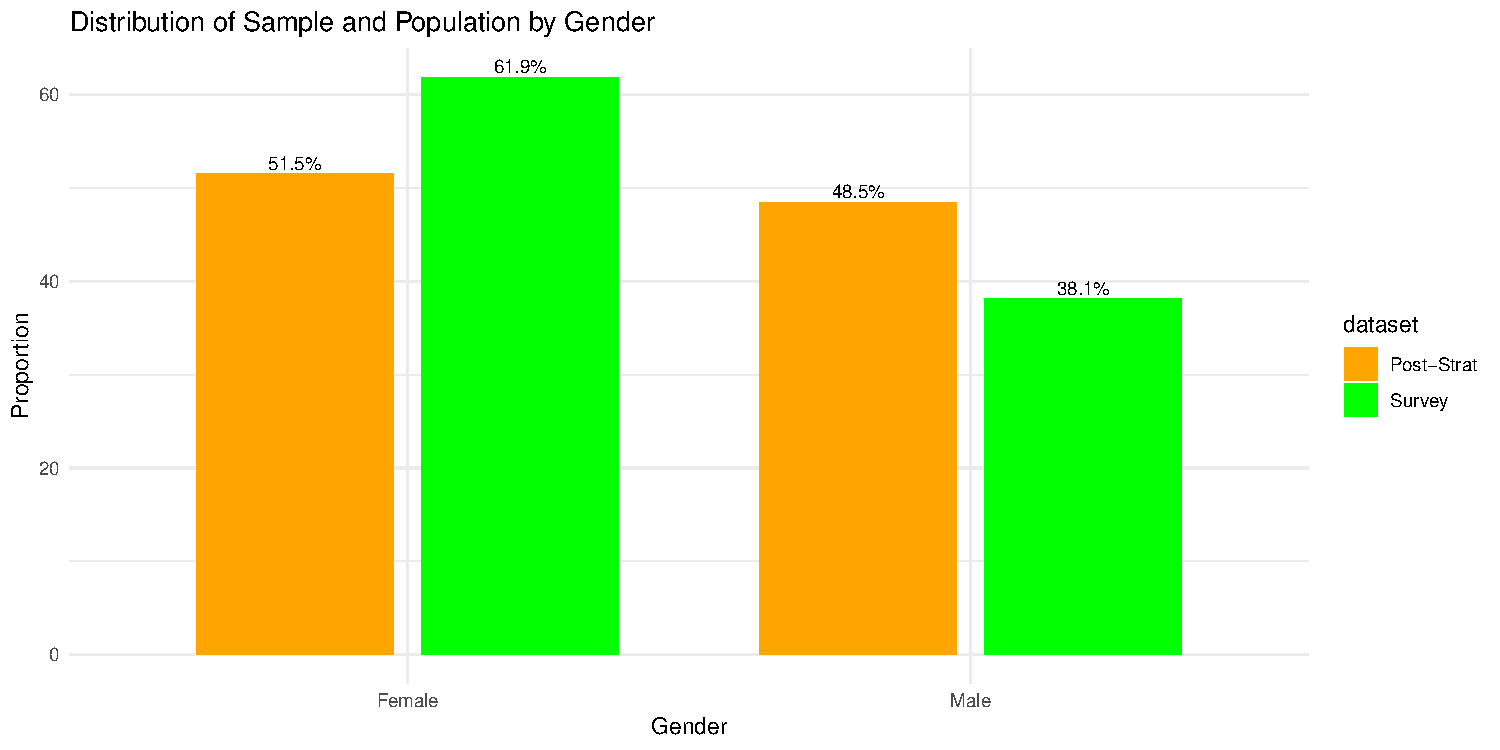
\includegraphics{paper_files/figure-pdf/fig-distribution-by-gender-1.pdf}

}

\caption{\label{fig-distribution-by-gender}Distribution of Sample and
Population by Gender}

\end{figure}

\begin{figure}

{\centering 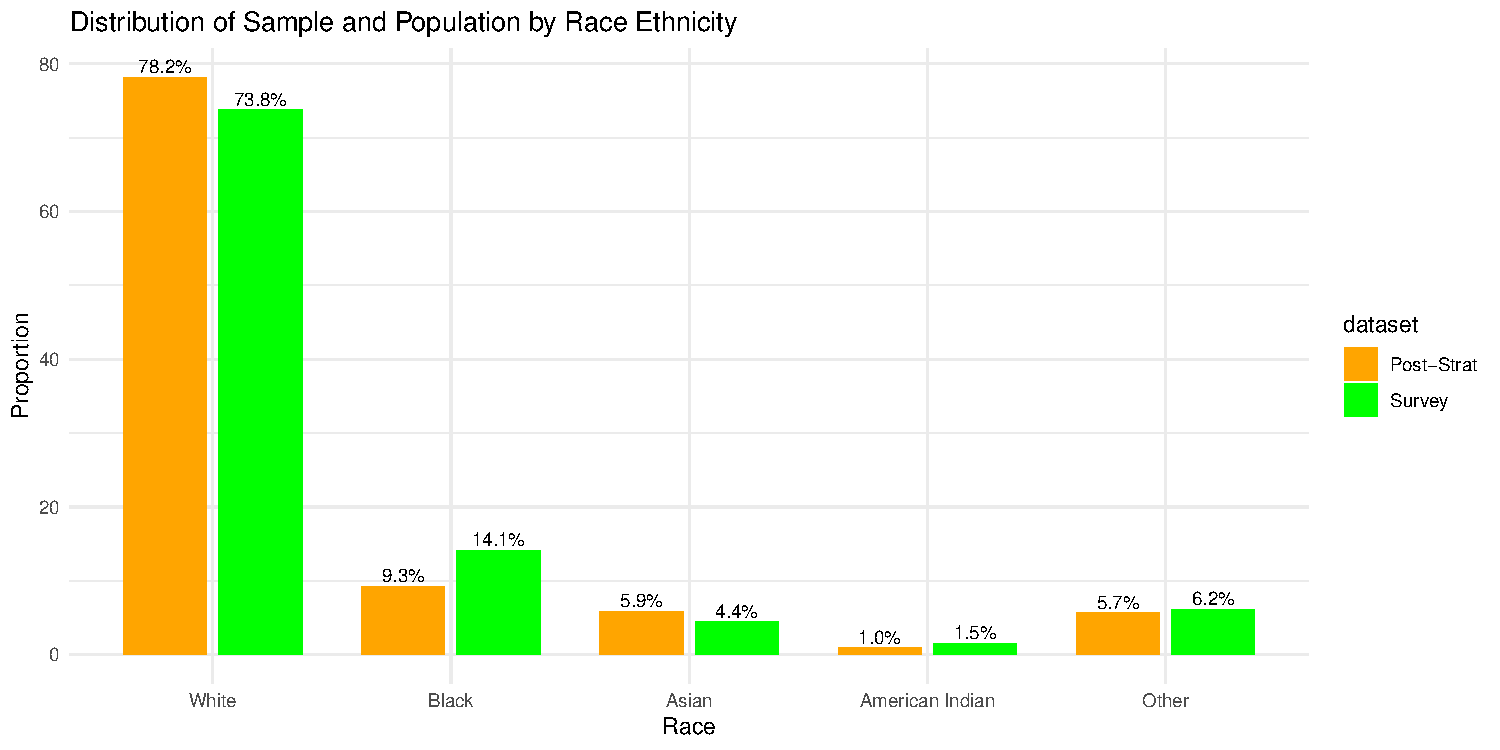
\includegraphics{paper_files/figure-pdf/fig-distribution-by-race-1.pdf}

}

\caption{\label{fig-distribution-by-race}Distribution of Sample and
Population by Race Ethnicity}

\end{figure}

\begin{figure}

{\centering 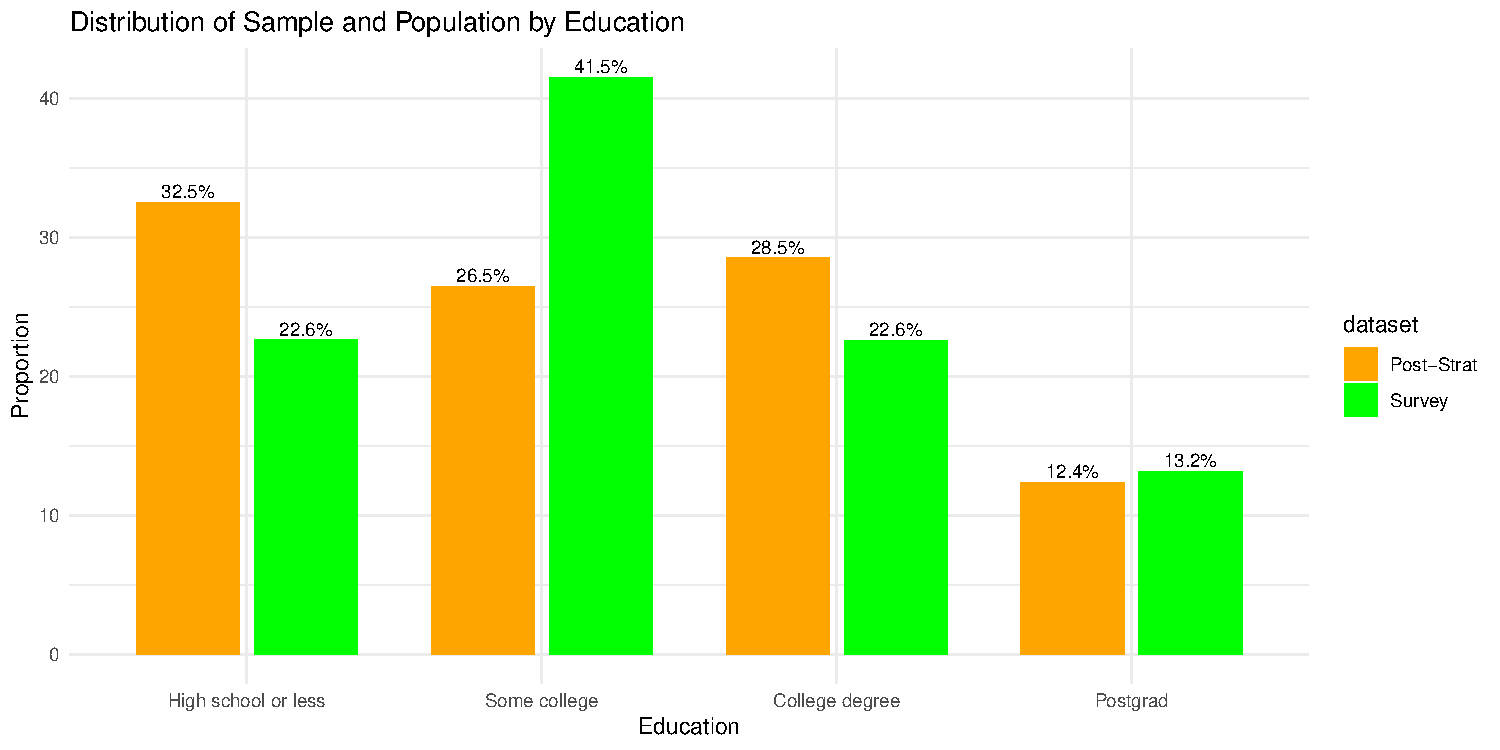
\includegraphics{paper_files/figure-pdf/fig-distribution-by-education-1.pdf}

}

\caption{\label{fig-distribution-by-education}Distribution of Sample and
Population by Education}

\end{figure}

\hypertarget{tbl-voters-intention-to-vote-for-trump}{}
\begin{table}[!h]
\caption{\label{tbl-voters-intention-to-vote-for-trump}Voters Intention to Support Trump }\tabularnewline

\centering
\resizebox{\ifdim\width>\linewidth\linewidth\else\width\fi}{!}{
\begin{tabular}{ccc}
\toprule
Response & Number of Respondents & Proportion (\%)\\
\midrule
\cellcolor{gray!10}{Yes} & \cellcolor{gray!10}{1908} & \cellcolor{gray!10}{34.25}\\
No & 3080 & 55.30\\
\cellcolor{gray!10}{Other} & \cellcolor{gray!10}{582} & \cellcolor{gray!10}{10.45}\\
\bottomrule
\end{tabular}}
\end{table}

\hypertarget{tbl-voters-intention-of-their-primary-party}{}
\begin{table}[!h]
\caption{\label{tbl-voters-intention-of-their-primary-party}Voters Intention of Their Primary Party }\tabularnewline

\centering
\resizebox{\ifdim\width>\linewidth\linewidth\else\width\fi}{!}{
\begin{tabular}{ccc}
\toprule
Party Preference & Number of Respondents & Proportion (\%)\\
\midrule
\cellcolor{gray!10}{Democratic} & \cellcolor{gray!10}{2180} & \cellcolor{gray!10}{39.14}\\
Republican & 1533 & 27.52\\
\cellcolor{gray!10}{Other} & \cellcolor{gray!10}{1857} & \cellcolor{gray!10}{33.34}\\
\bottomrule
\end{tabular}}
\end{table}

\hypertarget{model}{%
\section{Model}\label{model}}

For our study, we employ a technique called multilevel regression with
post-stratification (MRP). This approach involves creating a model based
on a smaller data set, such as our survey data, and then extending the
model's findings to a larger population.

\begin{longtable}[t]{lrrrr}
\caption{Coefficients from the Model}\\
\toprule
term & estimate & std.error & conf.low & conf.high\\
\midrule
(Intercept) & -1.13 & 0.82 & -2.59 & 0.19\\
genderMale & 0.65 & 0.06 & 0.55 & 0.74\\
educationHigh school or less & -0.02 & 0.09 & -0.18 & 0.13\\
educationPostgrad & -0.04 & 0.10 & -0.21 & 0.13\\
educationSome college & 0.13 & 0.08 & 0.00 & 0.26\\
\addlinespace
age\_group30-49 & 0.51 & 0.09 & 0.37 & 0.65\\
age\_group50-69 & 0.68 & 0.09 & 0.51 & 0.83\\
age\_group70+ & 0.90 & 0.13 & 0.69 & 1.11\\
raceAsian & -0.79 & 0.30 & -1.28 & -0.27\\
raceBlack & -1.71 & 0.28 & -2.15 & -1.24\\
\addlinespace
raceOther & -0.97 & 0.29 & -1.44 & -0.47\\
raceWhite & 0.19 & 0.25 & -0.21 & 0.61\\
stateAL & 0.18 & 0.83 & -1.15 & 1.66\\
stateAR & -0.07 & 0.83 & -1.44 & 1.40\\
stateAZ & -0.46 & 0.80 & -1.75 & 0.99\\
\addlinespace
stateCA & -0.58 & 0.79 & -1.85 & 0.84\\
stateCO & -0.41 & 0.82 & -1.75 & 1.05\\
stateCT & -0.90 & 0.87 & -2.27 & 0.61\\
stateDC & 0.13 & 0.94 & -1.46 & 1.74\\
stateDE & -0.03 & 0.92 & -1.55 & 1.57\\
\addlinespace
stateFL & 0.02 & 0.80 & -1.26 & 1.46\\
stateGA & 0.23 & 0.81 & -1.06 & 1.67\\
stateHI & -0.40 & 1.05 & -2.21 & 1.37\\
stateIA & -0.28 & 0.85 & -1.68 & 1.22\\
stateID & -0.57 & 0.91 & -2.12 & 1.02\\
\addlinespace
stateIL & -0.45 & 0.79 & -1.74 & 0.98\\
stateIN & -0.11 & 0.80 & -1.38 & 1.32\\
stateKS & -0.92 & 0.87 & -2.32 & 0.61\\
stateKY & 0.19 & 0.82 & -1.12 & 1.67\\
stateLA & 0.51 & 0.85 & -0.83 & 2.01\\
\addlinespace
stateMA & -1.01 & 0.81 & -2.33 & 0.43\\
stateMD & 0.25 & 0.82 & -1.05 & 1.71\\
stateME & 0.33 & 0.90 & -1.13 & 1.89\\
stateMI & -0.62 & 0.81 & -1.92 & 0.83\\
stateMN & -0.17 & 0.83 & -1.50 & 1.30\\
\addlinespace
stateMO & 0.26 & 0.82 & -1.03 & 1.72\\
stateMS & 1.00 & 0.86 & -0.34 & 2.50\\
stateMT & 0.92 & 1.04 & -0.75 & 2.74\\
stateNC & -0.32 & 0.80 & -1.64 & 1.13\\
stateND & -1.38 & 1.15 & -3.42 & 0.51\\
\addlinespace
stateNE & -0.74 & 0.85 & -2.17 & 0.79\\
stateNH & -1.16 & 1.00 & -2.83 & 0.53\\
stateNJ & -0.28 & 0.82 & -1.57 & 1.19\\
stateNM & 0.13 & 0.88 & -1.29 & 1.68\\
stateNV & -0.49 & 0.83 & -1.83 & 0.99\\
\addlinespace
stateNY & -0.40 & 0.79 & -1.69 & 1.03\\
stateOH & -0.28 & 0.80 & -1.55 & 1.17\\
stateOK & -0.55 & 0.82 & -1.89 & 0.91\\
stateOR & -0.61 & 0.84 & -1.98 & 0.88\\
statePA & -0.36 & 0.80 & -1.65 & 1.09\\
\addlinespace
stateRI & -0.87 & 0.96 & -2.46 & 0.80\\
stateSC & 0.05 & 0.83 & -1.26 & 1.50\\
stateSD & -0.13 & 1.00 & -1.73 & 1.58\\
stateTN & 0.08 & 0.81 & -1.22 & 1.55\\
stateTX & -0.11 & 0.79 & -1.37 & 1.34\\
\addlinespace
stateUT & 0.20 & 0.84 & -1.15 & 1.68\\
stateVA & -0.05 & 0.80 & -1.36 & 1.38\\
stateVT & -0.47 & 1.10 & -2.29 & 1.39\\
stateWA & -0.72 & 0.82 & -2.03 & 0.75\\
stateWI & -0.25 & 0.80 & -1.56 & 1.20\\
\addlinespace
stateWV & -0.16 & 0.88 & -1.56 & 1.36\\
stateWY & 0.82 & 1.03 & -0.85 & 2.57\\
\bottomrule
\end{longtable}

\hypertarget{model-set-up}{%
\subsection{Model set-up}\label{model-set-up}}

Define \(y_i\) as the number of seconds that the plane remained aloft.
Then \(\beta_i\) is the wing width and \(\gamma_i\) is the wing length,
both measured in millimeters.

\begin{align} 
y_i|\mu_i, \sigma &\sim \mbox{Normal}(\mu_i, \sigma) \\
\mu_i &= \alpha + \beta_i + \gamma_i\\
\alpha &\sim \mbox{Normal}(0, 2.5) \\
\beta &\sim \mbox{Normal}(0, 2.5) \\
\gamma &\sim \mbox{Normal}(0, 2.5) \\
\sigma &\sim \mbox{Exponential}(1)
\end{align}

We run the model in R (R Core Team 2023) using the \texttt{rstanarm}
package of Goodrich et al. (2022). We use the default priors from
\texttt{rstanarm}.

\hypertarget{results}{%
\section{Results}\label{results}}

\begin{table}

\end{table}

\begin{figure}

{\centering 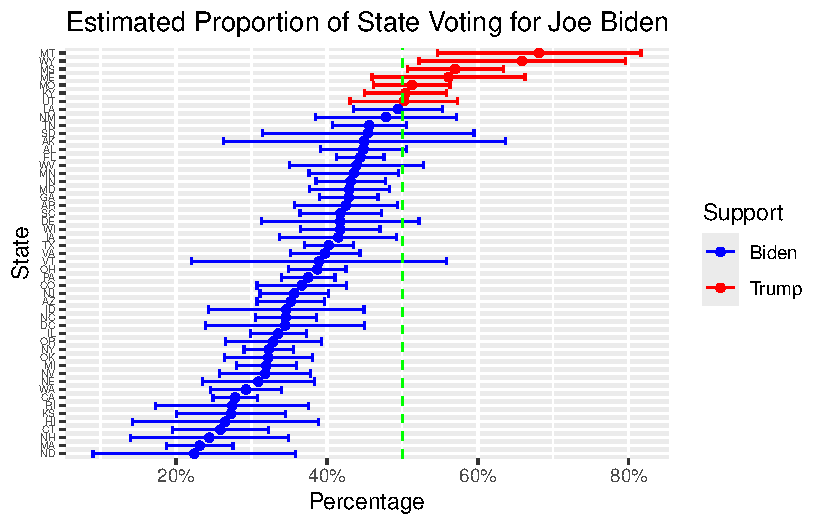
\includegraphics{paper_files/figure-pdf/stateplot-1.pdf}

}

\caption{Proportion of each State Voting for Trump}

\end{figure}

Figure @ref(fig:stateplot) shows us the estimated of proportion of
support for Trump and Biden by state using MRP with the inclusion of
error terms. Each dot represents the point estimate of the proportion of
support for Biden (blue) or Trump (red) in each state. Horizontal Lines
extending from the dots represent confidence intervals for these
estimates. The length of each line indicates the uncertainty associated
with each estimate. For instance, we can see that this uncertainty lies
between 50 percent to slightly higher than 80 percent for Trump in MT
(Massachusetts). The dashed green line in the middle at the 50 percent
mark represents the threshold for majority support. On the y-axis, each
state is listed with its abbreviations and is ordered based on the
proportion of support for Trump from the highest at the top to the
lowest at the bottom.

From figure @ref(fig:stateplot), it seems that majority of the states
support Biden. Only 7 states out of 51 have its point estimate greater
than 50 percent for Trump. However, the horizontal lines of confidence
intervals of some states overlapping the green mark give some hope for
the Republicans. However, excluding these contesting states, our model
suggests that only 3 states are definitely in favor of Trump whereas 35
states are definitely supporting Biden.

\begin{figure}

{\centering 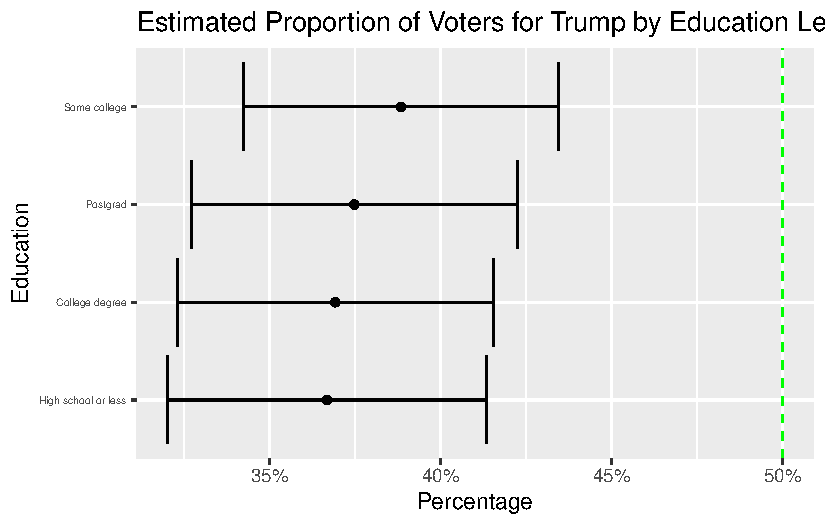
\includegraphics{paper_files/figure-pdf/educationplot-1.pdf}

}

\caption{How different education levels of voters affect voting for
Trump}

\end{figure}

Figure @ref(fig:educationplot) presents the estimated proportion of
voters for Trump by education level, divided into four categories: `High
school or less', `Some college', `College degree', `Postgrad'. Each
black dot represents the point estimate of the proportion of voters
within the corresponding education category who are predicted to vote
for Trump. The horizontal lines extending to the left and right of each
dot represent the confidence intervals around the estimate, which
reflect the uncertainty.

It shows that regardless of education level, the level of support for
Trump lies below 40 percent. The Republican party does not have
majority, including the error bars across all education levels. Voters
with ``High school or less'' education appear to have the lowest
estimated support for Trump, which does not align with various exit
polls and analyses from the 2020 election suggesting that Trump had
substantial support among voters without a college degree. Conversely,
Voters with `Some college' and `Postgrad' education are the two groups
that are more in support of Trump, which is exactly the opposite of what
we have expected.

\hypertarget{discussion}{%
\section{Discussion}\label{discussion}}

\hypertarget{sec-first-point}{%
\subsection{First discussion point}\label{sec-first-point}}

\hypertarget{second-discussion-point}{%
\subsection{Second discussion point}\label{second-discussion-point}}

\hypertarget{third-discussion-point}{%
\subsection{Third discussion point}\label{third-discussion-point}}

\hypertarget{weaknesses-and-next-steps}{%
\subsection{Weaknesses and next steps}\label{weaknesses-and-next-steps}}

Weaknesses and next steps should also be included.

\newpage

\appendix

\hypertarget{appendix}{%
\section*{Appendix}\label{appendix}}
\addcontentsline{toc}{section}{Appendix}

\newpage

\hypertarget{references}{%
\section*{References}\label{references}}
\addcontentsline{toc}{section}{References}

\hypertarget{refs}{}
\begin{CSLReferences}{1}{0}
\leavevmode\vadjust pre{\hypertarget{ref-rstanarm}{}}%
Goodrich, Ben, Jonah Gabry, Imad Ali, and Sam Brilleman. 2022.
{``Rstanarm: {Bayesian} Applied Regression Modeling via {Stan}.''}
\url{https://mc-stan.org/rstanarm/}.

\leavevmode\vadjust pre{\hypertarget{ref-Harris}{}}%
Harris, Adam. 2018. {``AMERICA IS DIVIDED BY EDUCATION.''} \emph{The
Atlantic}.
\url{https://www.theatlantic.com/education/archive/2018/11/education-gap-explains-american-politics/575113/}.

\leavevmode\vadjust pre{\hypertarget{ref-Prokop}{}}%
Prokop, Andrew. 2021. {``A New Report Complicates Simplistic Narratives
about Race and the 2020 Election.''} \emph{Vox}, May.
\url{https://www.vox.com/2021/5/10/22425178/catalist-report-2020-election-biden-trump-demographics}.

\leavevmode\vadjust pre{\hypertarget{ref-citeR}{}}%
R Core Team. 2023. \emph{R: A Language and Environment for Statistical
Computing}. Vienna, Austria: R Foundation for Statistical Computing.
\url{https://www.R-project.org/}.

\leavevmode\vadjust pre{\hypertarget{ref-citeSurveyData}{}}%
Tausanovitch, Chris, and Lynn Vavreck. 2020. \emph{Democracy Fund + UCLA
Nationscape}. October 10-17, 2019 (version 20200814).
\url{https://www.voterstudygroup.org/publication/nationscape-data-set}.

\leavevmode\vadjust pre{\hypertarget{ref-rohan}{}}%
Wickham, Hadley, Mara Averick, Jennifer Bryan, Winston Chang, Lucy
D'Agostino McGowan, Romain François, Garrett Grolemund, et al. 2019.
{``Welcome to the {tidyverse}.''} \emph{Journal of Open Source Software}
4 (43): 1686. \url{https://doi.org/10.21105/joss.01686}.

\end{CSLReferences}



\end{document}
